\documentclass[12pt,a4paper]{article}
% Use utf8
\usepackage[utf8]{inputenc}
% Define language
\usepackage[norsk]{babel}
% For images
\usepackage{graphicx}
% For hyperlinks
\usepackage{hyperref}

\def \fagkode{IT1901}
\def \fagtittel{Informatik Prosjektarbeid I}
\def \studentnummer{742414}
\def \gruppenummer{15}
\def \ordtelling{1857}
\def \tema{01 - Verktøy, sette opp miljøer}
\title{Rapport}

\begin{document}

\makeatletter
\begin{titlepage}
    \begin{center}
    
\includegraphics[width=0.60\textwidth]{NTNU_logo.png}\\[1cm]
    \textsc{\Large \fagkode}\\[0.5cm]
    \textsc{\large \fagtittel}\\[0.5cm]

    \rule{\linewidth}{0.5mm} \\[0.4cm]
    { \huge \bfseries \@title \\[0.4cm] }
    \rule{\linewidth}{0.5mm} \\[1.5cm]

    \LARGE
    \tema\\[1cm]

    \large
    Gruppe: \gruppenummer\\[0.25cm]

    \large
    Studentnummer: \studentnummer\\[0.25cm]

    \large
    Ordtelling: \ordtelling

    \vfill

    \large
    \@date
    \end{center}
\end{titlepage}
\makeatother

\newpage

\section*{Innledning}

Utviklermiljøer inneholder verktøy man trenger for å utvikle, analysere,
bygge og teste kode. Et minimalt utviklermiljø inneholder en text editor
og, avhengig av programmeringspråk, en kompilator eller interpreter.
Eksempelvis for C kan man bruke \texttt{vi} for å skrive kode og
\texttt{gcc} for å kompilere. Dette er helt fint brukbart til små
prosjekter og scripting.

Når man jobber med større prosjekter, er det nødvendig med flere
verktøy.

\section*{Verktøy for programvareutvikling}

Et sentralt verktøy i et prosjekt er et Package/Project Management Tool.
Dette er et verktøy som, blant annet, kan håntdere eksterne
avhengingheter, konfigurasjon og oppsett av prosjektet. Det finnes mange
verktøy i denne kategorien. Eksempelvis har man npm for
javascript-baserte prosjekter, composer for php, og gradle og maven for
java.

I IT1901 var prosjektet håndtert av Maven. Maven er et open source
prosjekt under Apache Foundation som sikter på å tilby en enkel og
uniform byggeprosess med høy kvalitet.\cite{maven}

Maven knyter sammen flere verktøy, plugins, som hver for seg utfører en
spesifikk oppgave. Prosjektet defineres av en project object model
(POM), som beskrives i xml-format. Når prosjektet er konfigurert,
trenger ikke utvikleren å vite detaljene rundt byggingen av prosjektet.
Dette øker kodekvaliteten da alle nødvendige sjekker gjøres automatisk
uten at utvikleren må vite hvilke verktøy som skal benyttes.

Byggeprosessen i maven består av flere faser, der hvert verktøy i tur
utfører sin oppgave:

\begin{itemize}
\item
  \texttt{validate} sjekker at alt av konfigurasjon er korrekt.
\item
  \texttt{compile} kompilerer kildekoden.
\item
  \texttt{test} utfører tester på den kompilerte koden.
\item
  \texttt{package} pakker den kompilerte koden inn i et distribuerbart
  format eksempelvis JAR.
\item
  \texttt{verify} gjør kodekvalitetsjekker og integreringstester.
\item
  \texttt{install} installerer pakken lokalt slik at den kan brukes som
  en avhengighet av andre lokale prosjekter.
\item
  \texttt{deploy} sender av gårde pakken til et eksternt repository slik
  at andre kan bruke prosjektet.
\end{itemize}

\subsection*{Kildekodehåndtering og versjonskontroll}

Versjonskontroll er verktøy som gjør håndteringen av kildekode enormt
mye enklere. Det fungerer ved å holde styr på endringer i kodebasen og
tilordner endringen et tidspunkt og en forfatter. Endringer kan deretter
enkelt sammenlignes med tidligere utgaver av koden, tilbakestilles
(restore/revert) hvis man ikke ønsker endringen likevel, og slås sammen
(merge) med andre endringer. Det finnes mange verktøy som utfører
versjonskontroll og kildekodehåndtering.

Noen versjonskontrollsystemer er innebygd i applikasjoner. Blant annet
har google implementert versjonskontroll i dokumenter i google drive.

Andre versjonskontrollverktøy er generelle og selvstendige, noen bruker
en server-client modell og andre er distribuerte. Eksempler på slike
verktøy er Concurrent Version System (CVS), Subversion (SVN) og GNU
Bazaar (bzr).

I dette kurset har vi brukt git for å håndtere kildekoden vår.
Git ble utviklet av Linus Torvalds i 2005 etter at forholdet mellom miljøet som utviklet linux-kjernen og det komersielle firmaet som utviklet deres daværende versjonskontrollverktøy, BitKeeper, surnet.
Det ikke eksisterte et (åpent) produkt som imøtekom behovene til utviklingen av linux-kjernen, og dermed laget Torvalds git.\cite{historyOfGit}

Git er et distribuert system,
som betyr at hele historien finnes lokalt på hvert enkelt filsystem
som har en kopi av koden;
hver kopi er en selvstendig og fullverdig utgave.

I tillegg måtte vi bruke GitLab, som er et grafisk web-basert verktøy,
for å interagere med git. Verktøyene som tilbys av GitLab faller mer
under prosjekthåndtering enn under versjonskontroll.

GitLab tilbyr, i tillegg til funksjonene til git, blant annet issue
tracking, som er et eget verktøy separat fra git. Det er et verktøy som
kan brukes for å beskrive, organisere, og tilordne oppgaver til
personer. GitLab kan også opprette branches basert på issues og
automatisk knytte commits til issues hvis issue nummeret nevnes i
commit-kommentaren.

\subsubsection*{Strategier for bruk av git}

I løpet av prosjektet har vi forsøkt å bruke git med forskjellige
strategier.

I starten benyttet vi oss av kun en branch, master branchen, og rebase
strategien for å sammenstille koden. Dette fungerer bra for små
iterative endringer og etterlater en lineær og lettleselig
endringshistorie. Målet med denne strategien var å unngå alt for mange
unødvendige og intetsigende merge commits i historien. Kombinert med
issue tracking er dette en ypperlig strategi hvis alle som jobber med
kodebasen er inneforstått med strategien og håndterer verktøyet.

\begin{figure}[ht]
    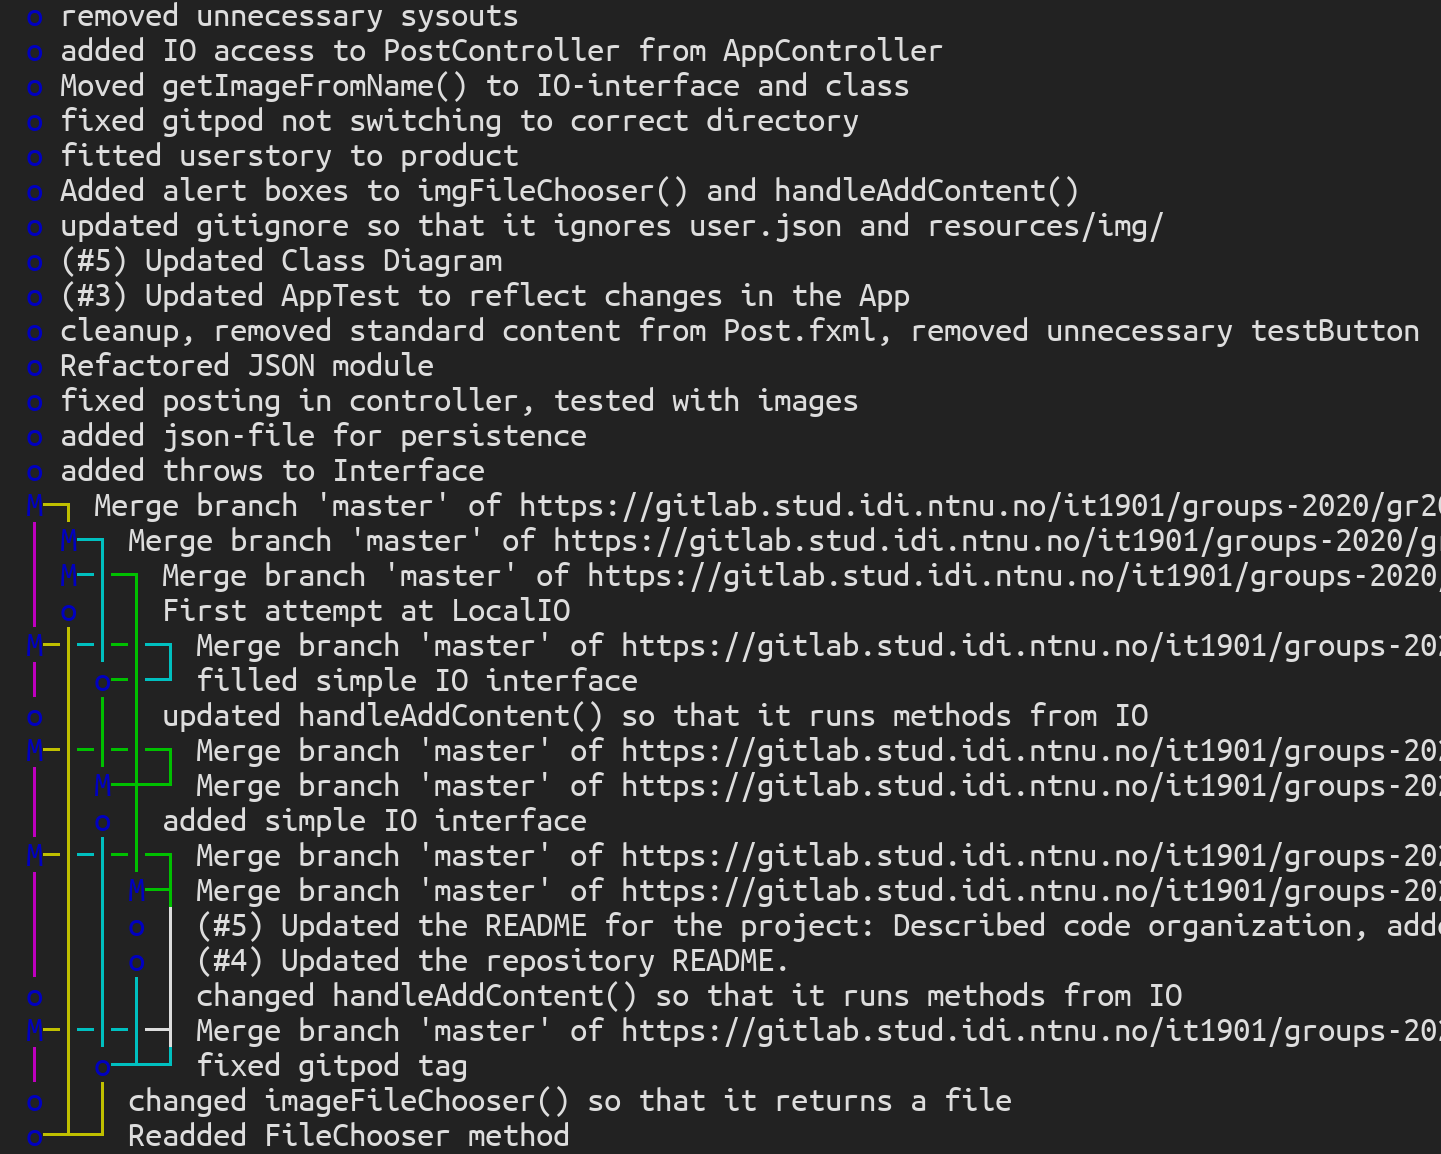
\includegraphics[width=\textwidth]{merge-rebase-example.png}
    \caption{Eksempel med merge før og rebase etter med nyere commits øverst i lista}
\end{figure}

Grunnen til at man kan bruke rebase på denne måten,
er at rebase skriver om historien. 
Når man rebaser en commit inn i en gren, lager git en ny commit med samme innhold.
\cite{gitEssentials}

En ulempe med å bruke rebase som strategi er at man potensielt kan havne
i lange kjeder av konflikter når man prøver å sammenstille forskjellige
endringer. Siden rebase prøver å plassere en commit der den kronologisk
hører hjemme, kan man ende opp med noen interessante og vanskelige
sammenstillinger.

\begin{figure}[ht]
    \centering
    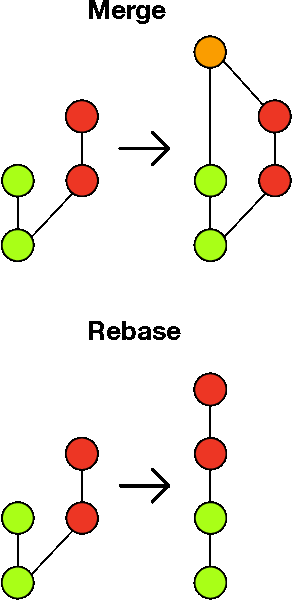
\includegraphics[width=0.33\textwidth]{git.png}
    \caption{Grafisk fremstilling av merge vs rebase. Med merge lages en ny commit for å sammenstille branchene, med rebase lages to nye commits på den første branchen.}
\end{figure}

Da innlevering nummer to sto for dør, ble vi tvunget til å benytte oss
av branches for kodingsoppgavene. Siden dette var et krav for oppgaven,
innrettet vi oss deretter. En av fordelene med å benytte oss av branches
var at vi kunne overta halvferdige implementasjoner fra andre i gruppa
uten at det måtte inn i master-branchen. En ulempe med dette var at det
var noe vanskeligere å implementere kode som avhenger av annen kode uten
å måtte sammenstille to uferdige branches.

Vi endte opp med å bruke en strategi som var en kombinasjon av de to
foregående. Hver branch representerer en (større) utviklingsoppgave og
alle sammenstillinger innenfor denne branchen brukte rebase som
strategi. Når en branch skulle sammenstilles med master branchen,
benyttet vi oss av merge strategien ved å gjøre en sammenstilling med
master før vi pushet upstream.

\subsubsection*{Konklusjon}

Etter å ha prøvd ut de forskjellige strategiene man kan bruke med git,
har jeg kommet frem til en følgende strategi som kan fungere bra for
prosjekterer av denne størrelsen: Små inkrementelle endringer kan gjøres
rett på master branchen med rebase strategien der commits merkes med
issue nummer. Større endringer (som vesentlig endrer arkitekturen
og/eller foregår over lengre tid med flere involverte) gjøres på en
branch forskjellig fra master og merges når endringen er klar. Dette
minimerer unødvendige og intetsigende merge commits i historien og
etterlater en lettleselig semi-lineær historie.

\subsection*{Statisk kodeanalyse}

Statisk kodeanalyse, i motsetning til dynamisk kodeanalyse, analyserer
koden uten å kjøre den.
De fleste IDEer og text editorer laget for kode
har innebygd linting, som er en form for statisk kodeanalyse som flagger
mulige feil i koden. Man kan si at stavekontroll er en form for linting
da grammatikk og stavefeil sjekkes.

Linting kan skje synkront, når man lagrer en fil eller manuelt kjører en
sjekk, eller asynkront når man skriver koden. Linting kan være så enkelt
som å la kompilatoren sjekke for syntaksfeil, eller det kan gjøres med
et verktøy som gjør en dypere analyse som også plukker opp logiske feil
i koden. Jeg brukte java-language-server, et open source-prosjekt som
blant annet utfører linting.

Gode verktøy for statisk analyse må være enkle å bruke;
de må gi forståelige tilbakemeldinger som vanlige dødelige utviklere kan forstå
så de kan skjønne hvilke feil de gjør og bli opplyst om hva god kodepraksis er.
Automatisert statisk kodeanalyse
er ikke en erstattning for code review utført av mennesker,
men heller en første sjekk som kan fremheve dårlig praksis
og deler av koden som trenger mer oppmerksomhet.
\cite{staticCodeAnalysis}

I vårt prosjekt benyttet vi oss også av kodeanalyseverktøyet SpotBugs.
Dette verktøyet oppdager vanlige feil og feller man kan gå i når man
skriver kode. Eksempelvis kan SpotBugs oppdage uendelige løkker og
variabler som aldri blir brukt til noe.

Tidlig i prosjektet valgte vi å ekskludere noen av reglene fra SpotBugs
da vi hadde noen ubrukte felter som skulle brukes i fremtiden. Dette
peker på dårlig planlegging av prosjektet og man kunne heller vært
flinkere på å gjøre ferdig en implementasjon heller enn å ha mange
halvferdige løsninger i kodebasen.

\subsection*{Kodeformatering}

Uniform kodeformatering bidrar til å gjøre kode mer lesbar
(men ikke nødvendigvis mer forståelig).
Det finnes mange verktøy som løser dette problemet.
Prettier er et prosjekt som støtter mange forskjellige språk
sentrert rundt front-end utvikling med npm som package managager.
Stylelint er et annet verktøy i denne kategorien
spesifikt rettet mot CSS/SCSS.

Argumentasjonen for bruk av denne typen verktøy ligner på den for LaTeX;
bruk mindre tid på å formatere innholdet og bruk mer tid på å skrive
innholdet. Hvis man automatiserer bruken av disse verktøyene, reduserer
man tiden som brukes på å formateringen og gir mer tid for
implementering. En annen fordel er at man unngår indenterings- og
whitespacekrig i versjonskontrollen.

Mange IDEer og text editorer støtter automatisk formatering ved hjelp av
disse verktøyene. Alternativt kan man bruke hooks i git for å automatisk
formatere koden før en commit. I verste fall kan man kjøre analyse med
verktøyet og manuelt ordne opp basert på tilbakemeldingen.

Vi valgte å bruke Checkstyle med google-java-format til å formatere
kildekoden vår. Det ble kjørt i \texttt{verify}-fasen av Maven og
rapporterte feil i formateringen. Ikke alle i gruppa brukte automatisk
formatering av koden, og brukte noe tid på å manuelt redigere koden for
å imøtekomme standarden. For å forbedre på dette kunne man ha brukt tid
i starten av prosjektet for å passe på at alle hadde et oppsett for
automatisk formatering eller lagt inn en pre-commit hook i repoet.

\subsection*{Testrapportering}

Testrapportering samler informasjon om hvilken del av kodebasen som har
blitt kjørt av automatiserte tester, og genererer en rapport som sier
noe om testdekningsgraden. En viktig ting å merke seg er at selv om
koden har kjørt under en test, betyr det ikke at koden er korrekt; det
kan fortsatt eksistere logiske feil i koden. Likevel er testdekning en
nyttig metrikk man kan bruke for å sjekke hvilken del av koden som er
testet.

Vi brukte Jacoco som er et slik verktøy. Det ble kjørt i
\texttt{verify}-fasen av Maven. Det ga oss bedre innsikt i hvilke deler
av koden som ble testet og hvilke deler som trengte ytterlige tester.

\section*{Konklusjon}

Ved å bruke de rette verktøyene i et programvareutviklingsprosjekt, kan
man sørge for at man skriver mer uniform og konsistent kode. Man øker
tilliten til at produktet man lager er robust og har færre feil. Riktig
bruk av versjonskontrollverktøy gjør at det er enkelt å samarbeide og
spore endringer og bidrag til prosjektet.

\newpage

\begin{thebibliography}{9}

    \bibitem{maven}
    \textit{What is maven?}\\
    \url{maven.apache.org/what-is-maven.html}

    \bibitem{historyOfGit}
    \textit{A Short History of Git}\\
    \url{https://git-scm.com/book/en/v2/Getting-Started-A-Short-History-of-Git}

    \bibitem{staticCodeAnalysis}
    Ivo Gomes, Pedro Morgado, Tiago Gomes, Rodrigo Moreira\\
    (2009) \textit{An overview of the Static Code Analysis approach in Software Developent}

    \bibitem{gitEssentials}
    Ferdinando Santacroce\\
    (2017) \textit{Git Essentials, Second Edition} Pact Publishing

\end{thebibliography}

\end{document}
